% start appendices FIXME
%%%%%%%%%%%%%%%%%%%%DO NOT MODIFY THIS PART%%%%%%%%%%%%%%%%%%%%%%%%%%%
\appendix
% \clearpage % or \cleardoublepage
\newpage
\makeatletter
\makeatother
\begin{appendices}
\chapter*{Appendix}
\addcontentsline{toc}{chapter}{}
% 밑의 sectioning이 ToC에서 보이고 싶은 느낌따라서,
% Appendix A.1 <-- \Alph
% Appendix 1.1 <-- \arabic 
% 중 선택하세요.
\renewcommand{\thesection}{\Alph{section}}
\renewcommand\thetable{\thesection.\arabic{table}}  
\renewcommand\thefigure{\thesection.\arabic{figure}}  
%%%%%%%%%%%%%%%%%%%%%%%%%%%%%%%%%%%%%%%%%%%%%%%%%%%%%%%%%%%%%%%%%%%%%%

\section{First Appendix}
\subsection{FIXME Appendix1}
\lipsum[1-2]~\cite{anderson1964hard}
\begin{figure}[!t]
	{
	\begin{center}
		\begin{tabular}{c}
			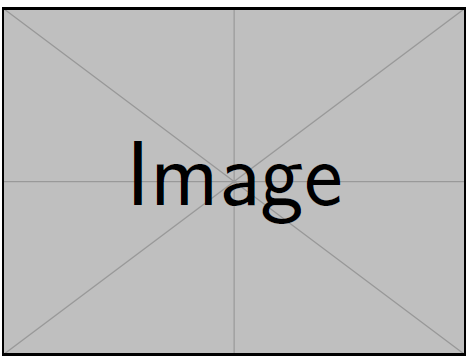
\includegraphics[width=0.9\linewidth]{dummy.png}
		\end{tabular}
	\end{center}
	}
	\caption[dummy image FIXME A1]{Figure option of $!\text{t}$.}
\label{dummy_imgA1}
\end{figure}
\subsection{FIXME Appendix2}
\begin{table}[htbp]
	\renewcommand{\arraystretch}{1.6}
	\setlength{\tabcolsep}{10pt}
	\caption{Table caption goes up FIXME A1}
	\label{tbl3_1}
	\centering
	\begin{tabular}{l l l l l l c}
	\hline\hline
	Material & $T_c$ & $B_c$& $\xi$ & $\lambda_L$ & $\kappa$ & Type \\
	\hfill & [K] & [T] & [nm] & [nm] & \hfill & \hfill \\
	\hline
	FIXME & 1 & 2 & 3 & 4 & 5 & FIXME \\
	\hline\hline
	\end{tabular}
\end{table}
\lipsum[1-2]~\cite{anderson1964hard}

\end{appendices}
% end appendices